\documentclass[12pt]{article}
\usepackage[utf8]{inputenc}
\usepackage{cite}
\usepackage[utf8]{inputenc}
\usepackage{graphicx}
\usepackage{amsmath}
\usepackage[margin=0.5in]{geometry}
\pagenumbering{gobble}
%\usepackage{geometry}
\usepackage{pdfpages}
\usepackage{xcolor}
\usepackage{todonotes}
\usepackage{amsmath,amsfonts,amssymb,amsthm,epsfig,epstopdf,titling,url,array}
\setcounter{secnumdepth}{4}
%\usepackage{enumerate}% http://ctan.org/pkg/enumerate
\title{Computational Model of Peri-Personal Space}
\author{Joan Reyero}
%\date{\today}


\bibliographystyle{apalike}
%\bibliography{bib}


\begin{document}

\maketitle

\section{Reinforcement learning models}

\subsection{Data exploration}

Before attempting to fit a model some data exploration was performed. Figure \ref{fig:2.1} shows the number of times each participant chose stimulus $A$, and the total number of rewards obtained. While participants who chose more times stimulus $A$ tend to have higher rewards, there is not a clear pattern observable in the figure. 

\begin{figure}[h!]
	\centering
	\hspace*{-0.6in}
	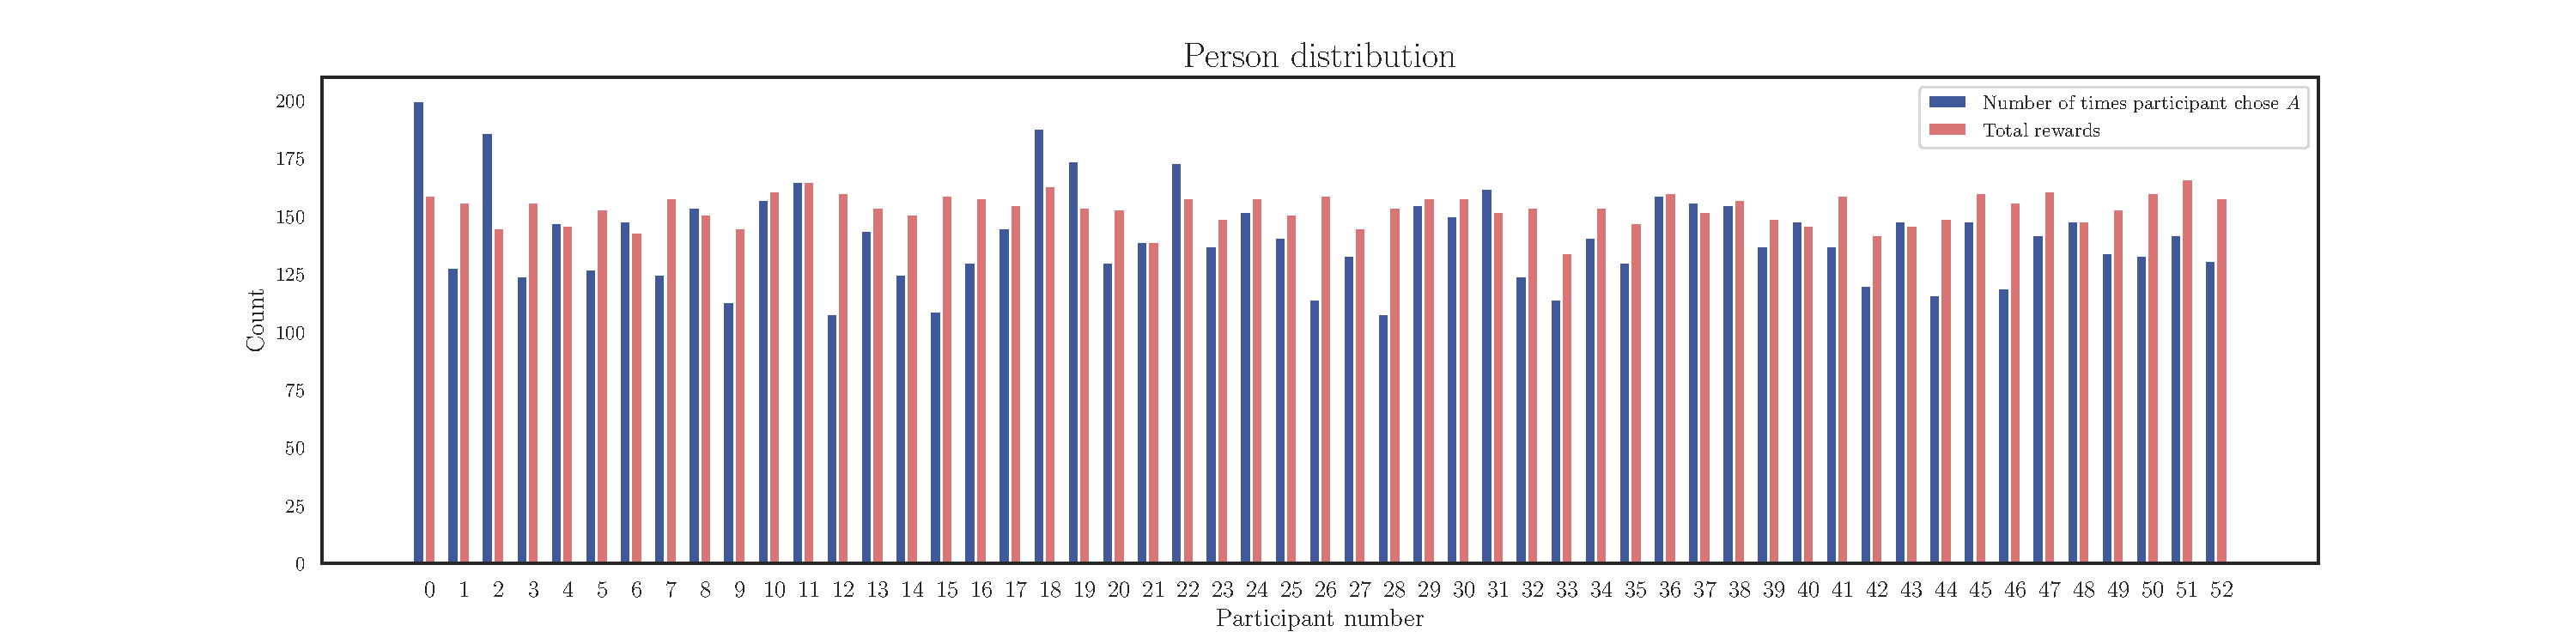
\includegraphics[width=1.2\linewidth]{figures/2.1.pdf}
	\caption{Plot of the total number of rewards and the number of times a participant chose stimulus $A$ for each participant.}
	\label{fig:2.1}
\end{figure}

The table below summarises the basic statistics for the studied variables. $A$ was chosen more than $50\%$ of the times, which is not surprising as, on average, choice $A$ had a higher probability of reward. The mean total rewards was 153.5, which is 64\% of the total.

The expected number of rewards if random choices were made can be obtained my

\[ \frac{\big(P(\mathrm{R} | A^1) + P(\mathrm{R} | B^1) + P(\mathrm{R} | A^2) + P(\mathrm{R} | B^2)\big) \times 100}{4} = 56.25 \]

Therefore, the expected number of rewards is lower than the average rewards obtained, which suggests that learning happened during the experiment.

\begin{center}
 \begin{tabular}{|c || c | c | c|} 
 \hline
  & Mean (out of 240) & Standard deviation & Range (out of 240) \\ [0.5ex] 
 \hline\hline
 Times $A$ was chosen & 141.0 & 20.31 & $[108, 200]$ \\ 
 \hline
 Total rewards & 153.5 & 6.63 & $[134,166]$ \\ [1ex] 
 \hline
\end{tabular}
\end{center}



\bibliography{bib}

\end{document}
